\documentclass[output=paper]{langscibook}
\ChapterDOI{10.5281/zenodo.5483100}

\author{Izabela Jordanoska\affiliation{University of Vienna} and Erlinde Meertens\affiliation{University of Konstanz}}
\title[The pragmatic effects of Macedonian \textup{li}: An empirical study]
      {The pragmatic effects of Macedonian \textit{li}: An empirical study}
\abstract{In this paper we provide empirical data concerning the  pragmatics of the particle \textit{li} following nominal phrases in polar questions in Macedonian. Since in previous literature \textit{li} has been analyzed as a focus particle, we put forward two hypotheses on its effect in questions that can follow from focus marking: (i) that \textit{li} signals uniqueness of the entity that is denoted by the constituent it is attached to or (ii)~that \textit{li} signals surprise about the entity denoted by the constituent it is attached to. We have conducted an online survey that shows that polar questions in which \textit{li} is adjacent to a fronted XP are felicitous in contexts containing surprise, regardless of whether that XP is unique or not. We account for these findings using questions under discussion and alternative semantics.
%  \textit{li} in Macedonian that helps us investigate what \textit{focus marking} using the particle \textit{li} in polar questions Macedonian exactly contributes.

\keywords{question particles, semantics, pragmatics, focus, Macedonian}
}



\begin{document}
\maketitle

\section{Introduction}

This paper is concerned with the semantic-pragmatic conditions for the seemingly optional particle \textit{li}, which, in Standard \ili{Macedonian} (Eastern South \ili{Slavic}; henceforth just \ili{Macedonian}), mostly appears in polar questions.

There are at least six ways of forming polar questions in \ili{Macedonian}, involving interaction between word order, intonation, and the particle \textit{li}, as illustrated in \REF{bigli}.\footnote{If not indicated otherwise, all examples are from \ili{Macedonian}.}\textsuperscript{,}\footnote{Other environments in which \textit{li} can appear, albeit rarely, are habitual conditionals in \REF{cond}, content questions in \REF{sto}, alternative questions in \REF{altq} and a special kind of duratives in \REF{dur}. We mention these here for completeness.
\ea
\ea \gll Mine li, gori zemja-ta.\\
    pass.by.\textsc{prs.3sg} \textsc{li} burn.\textsc{prs.3sg} earth-\textsc{def.sg.f}\\
    \glt `Whenever/if (s)he walks by, the earth burns.' \label{cond} \hfill  \citep[539]{koneski1987}
        \ex \gll Što li najde vo nego? \\
what \textsc{li} find.\textsc{prs.3sg} in \textsc{3sg.m.dat.pro} \\
\glt `Whatever did (s)he see in him?!' \label{sto} \hfill  \citep[561]{Rudin.Kramer.Billings.Baerman1999}
        \ex  \gll Malini li se, kapini li se? \\
raspberry.\textsc{pl} \textsc{li} be.\textsc{prs.3pl} blackberry.\textsc{pl} \textsc{li} be.\textsc{prs.3pl} \\
\glt `Are they raspberries, or are they blackberries?' \label{altq}  \hfill  (heard in conversation July 2018)
        \ex \gll Tamu vetar-ot duva li duva! \\
there wind-\textsc{def.sg.m} blow.\textsc{prs.3sg} \textsc{li} blow.\textsc{prs.3sg} \\ \glt
`There the wind keeps blowing and blowing!'  \label{dur} \hfill (heard in conversation August 2019)

\z\z}

% Example 1

\ea
    \ea \gll Saka-š musli? \\
want-\textsc{prs.2sg} muesli \\ \hfill Intonation question (IntQ)\label{intonation}
\glt  `Do you want muesli?' \label{intoq}
    \ex \gll Dali saka-š musli? \\
\textsc{q} want-\textsc{prs.2sg} muesli \\ \hfill Dali question (DaliQ)
\glt `Do you want muesli?'  \label{dali}
    \ex \gll Musli li saka-š? \\
muesli \textsc{li} want-\textsc{prs.2sg} \\ \hfill XP-li question (XP-LiQ)\label{li}
\glt `Do you want \emph{muesli}?'\footnote{We use prosodic prominence, indicated with capitals, as the equivalent of \textit{li} in the English translations. Though prosody also plays a role in \ili{Macedonian}, we make no claims about it in this paper.}
    \ex \gll Musli, saka-š li? \\
muesli want-\textsc{prs.2sg} \textsc{li} \\ \hfill Topic question (TopQ)
\glt `As for muesli, \emph{do} you want it?'\label{topli}
    \ex \gll Saka-š li musli? \\
want-\textsc{prs.2sg} \textsc{li} muesli \\ \hfill V-li question (V-LiQ)
\glt `\emph{Do} you want muesli?' \label{vli}
    \ex \gll Musli e toa što saka-š? \\
muesli be.\textsc{prs.3sg} that what want-\textsc{prs.2sg} \\ \hfill Cleft question (CleftQ)
\glt `Is it muesli that you want?'\\ \label{cleft} \hfill (based on the examples in \citealt[579]{Rudin.Kramer.Billings.Baerman1999})
\z\z \label{bigli}

% \begin{exe} \ex \begin{xlist}
% \ex \gll  Ima Pepsi? \\
%  have.\textsc{3sg} Pepsi \\ \trans
%     `Is there pepsi?' \hfill [Intonation question (IntQ)] \label{intonation}
% \ex \gll Dali ima Pepsi? \\
%     Q have.3sg Pepsi \\ \trans
%     `Is there Pepsi?' \hfill [Dali question (DaliQ)] \label{dali}
% \ex \gll Pepsi li ima? \\
%     Pepsi \textsc{li} have.\textsc{3sg} \\ \trans
%     `Is there PEPSI?'  \hfill [XP-li question (LiQ)]  \label{li}
%     \ex \gll Pepsi, ima li? \\
% Pepsi have-\textsc{3sg} \textsc{li} \\ \trans
% `As for Pepsi, IS it there?'\hfill [Topic question (TopQ)]
% \ex \gll Ima li Pepsi? \\
% have-\textsc{3sg} \textsc{li} Pepsi \\ \trans
% `IS there Pepsi?'
% \end{xlist} \end{exe} \label{bigli} \\based on the examples in \citep[579]{Rudin.Kramer.Billings.Baerman1999}
\noindent
In \REF{intoq} the polar question is neither marked by word order, which remains SVO, nor by any particle, but solely by intonation. In \REF{dali} the word order remains canonical, but the question particle \textit{dali} appears clause-initially. This is interpreted as a neutral question.
Whenever \textit{li} occurs, it always cliticizes to the first constituent of the clause; this constituent may only be preceded by a topic. In \REF{li} the first constituent is the fronted XP \textit{musli}. In both \REF{topli} and \REF{vli} \textit{li} attaches to the verb. In \REF{topli} the object \textit{musli} has been topicalized, making it appear before the verb. Finally, \REF{cleft} is a cleft question. It is unclear what the differences in usage between the questions in \REF{bigli} are, though some suggestions, to be discussed in \sectref{sec:back}, have been made. To our knowledge, no empirical work on the usage of the different question types in colloquial language is available.\footnote{See \citet{englund1977} for a corpus study of literary works.} In order to get a step closer towards both filling this empirical gap and gaining understanding of the mea\-ning contribution of \textit{li}, we present the findings of an empirical study that provide insights in the usage conditions of XP-LiQs, such as \REF{li}. More precisely, we show that XP-LiQs are felicitous in contexts that trigger \textsc{surprise}.

The structure of the paper is as follows. We discuss previous literature and formulate our hypotheses in \sectref{sec:back}. \sectref{sec:method} and \sectref{sec:results} serve to describe the methodology and results. In \sectref{sec:analysis} we interpret our results and work towards an analysis. We conclude in \sectref{j:sec:conclusion}.
%%%%%%%%%%%%%%%%%%%%%%%%%%%%%%%%%%%%%
%       Section 2
%%%%%%%%%%%%%%%%%%%%%%%%%%%%%%%%%%%%%
\section{Background and hypotheses}\label{sec:back}

In this section we discuss previous approaches to XP-LiQs, leading us to formulate two hypotheses about the meaning contribution of \textit{li}. We then elaborate on the semantic assumptions and predictions of both hypotheses.

Several suggestions on the pragmatic contribution of \textit{li} have been put forward in the literature. First of all, \citet{minova1987} and \citet{Rudin.Kramer.Billings.Baerman1999} have reported that XP-LiQs are interpreted as rhetorical questions. Moreover, \citet{Rudin.Kramer.Billings.Baerman1999} have put forward that V-LiQs convey surprise. This observation is shared by \citet[137]{lazarova2003},  who claims that \textit{li} ``adds a tone of surprise to the focused constituent'' and shows this with a V-LiQ example. A third observation comes from \citet{englund1977}, namely that XP-LiQs expect ``no'' as an answer. In contrast, \citet{kramer1985}, as cited in \citet{Rudin.Kramer.Billings.Baerman1999}, has examples of IntQs, DaliQs and XP-LiQs being acceptable in the same situations. All three, for example, can be used when asking a shopkeeper if they have a certain product, suggesting that whatever difference there is between them is minimal. Finally, \citet{koneski1965}, as cited in \citet[128]{englund1977}, has noted that there is also regional variation, with \textit{li} questions being more rare in Western dialects. Though our survey is concerned with Standard \ili{Macedonian}, which is based on West Central dialects \citep{Friedman2001}, most of our participants were from either Skopje, where West Central dialects are spoken, or Štip, where Eastern dialects are spoken (see \sectref{sec:methodp}).

While these suggestions have not been systematically explored, there is consensus in the literature that
\textit{li} is associated with \textsc{focus marking}, as the constituent it is adjacent to is focus-fronted \citep{Tomic1996a, Rudin.Kramer.Billings.Baerman1999,schwabe2004,lazarova2003}. The cited papers focus on the syntax and phonology of \textit{li} and say little about its usage. The aim of this paper is to investigate the pragmatic effects of focus on polar questions.

It is widely accepted and agreed upon that the semantic and pragmatic effect of focus in declaratives is to generate a set of alternatives \citep{rooth1992}.  The pragmatic contribution of focus in questions, such as \REF{didjohn}, is less understood.
%onsider the English sentence in (\REF{john}).

% \begin{exe}
% \ex JOHN played cards. \label{john}
% \end{exe}

% Example 2

\ea Did \emph{John} play cards? \label{didjohn}
\z

% The focus semantic value $\llbracket . \rrbracket^{f}$ for a declarative, such as `ALI played cards' is exemplified in \REF{play}, and the focus felicity condition of the squiggle operator $\thicksim$ is defined in \REF{def}.

% \begin{exe} \ex
% \begin{xlist}
% \ex  $\llbracket $Ali\textsubscript{F} played cards$\rrbracket$ = \{ a played cards, b played cards, c played cards \}\label{play}
% \ex $\llbracket \phi \thicksim $C$\rrbracket$ is felicitous only if $\llbracket$C$\rrbracket \subseteq \llbracket \phi \rrbracket^{f}$ \label{def} \end{xlist} \end{exe}
\noindent
For questions, one possible analysis is that -- employing \textsc{questions under discussion} (QUD, \citealt{Roberts2012}) and \textsc{discourse trees} \citep{Buering2003} -- focus in questions indicates a sub-question in a discourse strategy \citep{biezma2009, kamali.buering2011}. This analysis will be elaborated on in \sectref{sec:analysis}.
%Thus the super-question of \REF{didjohn} is `Who played cards?', as illustrated in \REF{cards}.

% \begin{exe}
% \ex \label{roberts8}
% {\scriptsize
% \Tree [.{Who played cards?} [{Did JOHN play cards?} {Did ALI play cards?} ... ]. ]} \label{cards}
% \end{exe}

The issue remains what motivation the speaker can have to make the sub-question explicit.
We formulate two hypotheses which can be accounted for by a QUD analysis of focus in questions: that the speaker makes the sub-question explicit to indicate that what is denoted by the \textit{li}-marked constituent is either unique, or that they are surprised about it. The hypotheses are given in \REF{hyp}.\footnote{We thank Radek Šimík for useful feedback on our definition of \textit{uniqueness}.}

% Further suggestions as to the pragmatics of LiQs are:
% i) In a corpus study of \ili{Macedonian} literary works \citet{englund1977yes} has found that \textit{dali} is more likely to appear in questions which expect `yes' as an answer, whereas \textit{li} is better with questions that expect `no' as an answer.
% ii) \citet{minova1987partikulata} says that negative LiQs are often rhetorical and \citet{Rudin.Kramer.Billings.Baerman1999}'s consultants also reported positive LiQs to have a rhetorical flavour. Interestingly, according to \citet{Rudin.Kramer.Billings.Baerman1999}, in \ili{Bulgarian} it are the DaliQs, which in \ili{Macedonian} are considered neutral, that are more likely to be interpreted as rhetorical.

% On the other hand, \citet{kramer1985anglisko}, as cited in \citet{Rudin.Kramer.Billings.Baerman1999}, has examples of IntQs, DaliQs and LiQs being acceptable in the same situations. All three, for example, can be used when asking a shopkeeper if they have a certain product, suggesting that whatever difference there is between them is minimal.

%  Finally, there is regional variety to take into account. The eastern dialects, which are closer to \ili{Bulgarian}, employ \textit{li} more often than the Western ones \citep{koneski1965recnik}, \citep{englund1977yes}.
%  While this is not the main question of our research, it is something we take into account in a post-hoc analysis.


%  In this paper we provide empirical data concerning the usage of \textit{li} in \ili{Macedonian} that helps us understand the various observations on the usage of \textit{li} discussed in \REF{sec:back}
%  and investigate what \textit{focus marking} using the particle \textit{li} in polar questions \ili{Macedonian} exactly contributes.

% Based on the observations above

% Example 3

\eanoraggedright\label{hyp}
\eanoraggedright Hypothesis 1:\\
XP-LiQs signal that there is a property (or entity) in our world which uniquely satisfies the property (or entity) that is denoted by the \textit{li}-marked constituent (i.e. there is one unique value of the type of the \textit{li}-marked constituent that will make the proposition that is denoted by the question true). \label{hyp1}
\ex Hypothesis 2:\\ XP-LiQs signal that the speaker is \textsc{surprised} about the property (or entity) denoted by the \textit{li}-marked constituent. \label{hyp2}
\z\z

\noindent
The motivation for these hypotheses is elaborated in the following two sections.

%%%%%%%%%%%%%%%%%%%%%%%%%%%%%%%%%%%%%%%%
% Subsection 2.1

\subsection{Hypothesis 1: `Uniqueness'}\label{sec:uniqueness}

The first hypothesis is that XP-LiQs signal that the property (or entity) that is denoted by the \textit{li}-marked constituent is unique. A definition of uniqueness is given in \REF{uniqueness}.

% Example 4

\ea \textsc{uniqueness}: there is only one possible relevant $x_{\langle e \rangle}$ under discussion. \label{uniqueness}
\z

\noindent
This is reminiscent of (pseudo-)cleft constructions, such as \REF{cleft}, repeated here as \REF{cleft2}, which, at least for English, are said to have a uniqueness presupposition (\citealt{drenhaus2011}, among others).

% Example 5

\ea \gll Musli e toa što saka-š? \\
muesli be.\textsc{prs.3sg} that what want-\textsc{prs.2sg} \\
\glt `Is it muesli that you want?'
\label{cleft2}
\z

\noindent
Support for this hypothesis comes from \citeposst{dukova2010} analysis of focus in questions in \ili{Bulgarian}. \ili{Bulgarian}, being an Eastern South \ili{Slavic} language, is closely related to \ili{Macedonian}. \citet{dukova2010} claims that XP-LiQs contain a presupposition, as they involve a contrastive focus. An example to illustrate this is given in \REF{ivan}.

% Example 6

\eanoraggedright
\eanoraggedright \textit{Scenario}: Paul, Ivan, Mary, Susan and Peter are students of history. Usually their final
examinations are oral. Today they have an examination of this type. The teacher is in her
office and asks them to enter one by one. The exam has just begun. Paul is in the teacher's
office, when Peter's phone rings. In order to not disturb his classmates, Peter moves away to
answer the call. A few minutes later he comes back, but he sees only Mary and Susan's purse.
He asks then if the one who has entered next is Ivan, thinking that Susan is probably
somewhere else since she has left her things.
\ex \gll Ivan li vleze? \\
Ivan \textsc{li} enter.\textsc{prs.3sg} \\
\glt `Is Ivan the one who entered?' \hfill (\ili{Bulgarian};  \citealt[258]{dukova2010})
\label{ivan}
\z\z

\noindent
The translation of \REF{ivan} as a cleft question in English is already hinting at a uniqueness interpretation. The context \citet{dukova2010} sets up for \REF{ivan} is such that only one person can be in the room at the same time, i.e., there is only one relevant person under discussion. The alternatives for \REF{ivan} are `Is Bill the one who entered?', `Is Susan the one who entered?', etc. Furthermore, translating sentences with XP-\textit{li} as cleft questions is also employed by \citet{king1994} for \ili{Russian}.

% Furthermore, frontend foci with \textit{li} are also translated as clefts by King for \ili{Russian} and bla for \ili{Finnish} (as cited in \citep[3]{bianchi2016derivation}

% Furthermore, in \ili{Turkish}, when the question particle \textit{mI} is adjacent to the stressed constituent, it gets an exhaustive interpretation \citet{kamali2011topics}.

\subsection{Hypothesis 2: `Surprise'}\label{sec:surprise}
A second hypothesis for the effect of focus in XP-LiQs is that XP-\textit{li} signals surprise rather than uniqueness. Motivations for this hypothesis are first of all the observations by \citet{Rudin.Kramer.Billings.Baerman1999} and \citet{lazarova2003} that, at least for V-LiQs, \textit{li} adds a surprise flavor to a question, as mentioned in \sectref{sec:back}.

% One possible reason comes from \citep{bianchi2016focus}, who have said focus in questions in signals \textit{surprise} or \textit{mirativity}, this will be further elaborated on in section \REF{sec:surprise}. For \ili{Macedonian}, both \citet{Rudin.Kramer.Billings.Baerman1999} and \citet{lazarova2003interrogative} have mentioned that \textit{li} adds a feeling of surprise.

Furthermore, \citet{bianchi.cruschina2016} and \citet{bianchi.bocci.cruschina2016} have found that in \ili{Sicilian}, and several other languages, polar questions with a fronted focus can be interpreted as having a \textsc{mirative import}, i.e., that ``there is at least one alternative proposition which is more likely than the asserted one'' \citep[60]{bianchi.cruschina2016}.

The definition of surprise we used in this experiment is a mismatch between a negative \textsc{epistemic bias}  and a positive \textsc{evidential bias}. \citet{sudo2013}, building on \citeposst{buering.gunlogson2000} concept of \textsc{contextual evidence}, proposes these two types of bias in order to account for certain \ili{Japanese} biased question particles.
Epistemic bias contains the expectations based on world knowledge and speakers' beliefs, whereas evidential bias is contextual evidence gained from direct observations. An example to illustrate these concepts in English is given in \REF{smoke}.

% Example 7

\ea
\ea Do athletes smoke?
\ex \textsc{(negative) epistemic bias}: Athletes don't smoke cigarettes.
\ex \textsc{(positive) evidential bias}: You see an athlete smoking a cigarette.
\z \label{smoke} \z

\noindent
In order to find out which of these two hypotheses holds, we have set up a questionnaire, the details of which are shown in the next section.
%%%%%%%%%%%%%%%%%%%%%%%%%%%%%%%%%%%%%
%       Section 3
%%%%%%%%%%%%%%%%%%%%%%%%%%%%%%%%%%%%%
\section{Methodology}\label{sec:method}

\subsection{Design}\largerpage
We tested our hypotheses in a rating study. Two factors were manipulated. First, the form of the target question, which came in three conditions: XP-LiQ, DaliQ and CleftQ. The second factor was the context type, which also came in three conditions: Unique\,+\,Surprise, Non-unique\,+\,Surprise and Neutral.

27 experimental items were distributed in 7 lists with a Latin square design, together with 8 fillers that served as controls. Each trial consisted of a context and a question.
Participants were asked to rate the naturalness of a question in a context on a 1 (min)--5 (max) Likert scale. They were given two test trials before the actual trials. The survey was conducted online using SoSci Survey \citep{leiner2014}.


 \subsection{Stimuli}
 The stimuli were presented in written form in \ili{Macedonian} Cyrillic.\footnote{For practical purposes, we only make use of the Latin transliteration in this paper.} An example of a Unique\,+\,Surprise context is given in \REF{unisur}.

% Example 8

\eanoraggedright
\eanoraggedright \textsc{uniqueness\,+\,surprise}: Your friend bought a necklace with a precious stone. You don’t recognize the stone, but you are sure it isn't ruby, because it is not red. Then your friend starts talking about how expensive ruby is. You ask her: \label{unisur}
    \ex \gll Rubin li ima vo ǵerdan-ot? \\
ruby \textsc{li} have.\textsc{prs.3sg} in necklace-\textsc{def.3sg.m} \\ \hfill XP-LiQ
\glt `Is there \emph{ruby} in the necklace?'  \label{rubinli}
    \ex \gll Dali ima rubin vo ǵerdan-ot? \\
\textsc{q} have.\textsc{prs.3sg} ruby in necklace-\textsc{def.3sg.m} \\ \hfill DaliQ
\glt `Is there ruby in the necklace?'  \label{dalirubin}
    \ex \gll Rubin e toa što e vo ǵerdan-ot? \\
ruby be.\textsc{prs.3sg} that what be.\textsc{prs.3sg} in necklace-\textsc{def.3sg.m} \\ \hfill CleftQ
\glt `Is it ruby that is in the necklace?'  \label{cleftrubin}
\z\z

\noindent In \REF{unisur} there is only one stone in the necklace, hence uniqueness. Surprise is present in the context because the speaker has an epistemic bias that there are no rubies in the necklace, when suddenly their friend mentions ruby in relation to the necklace, reflecting a positive evidential bias.
This context was presented with either a XP-LiQ, as in \REF{rubinli}, a DaliQ, as in \REF{dalirubin} or a CleftQ, as in \REF{cleftrubin}. A Non-unique\,+\,Surprise context is given in \REF{nonunisur}, where the set-up for surprise is the same, but crucially, there are now multiple stones in the necklace and none of them is singled out by the context.

% Example 9

\eanoraggedright \textsc{non-uniqueness\,+\,surprise:} Your friend bought a necklace with multiple precious stones, such as amethyst, sapphire, pink quartz and some more. You think it doesn't contain ruby, because none of the stones is red. Then your friend starts talking about how expensive ruby is. You ask her: [...] \label{nonunisur}
\z

\noindent
\REF{neut} is an example of a neutral context, in which there is no set-up for surprise and there are multiple precious stones under discussion.

% Example 10

\eanoraggedright
\textsc{neutral:} Your friend bought a necklace with multiple precious stones, such as amethyst, sapphire, pink quartz and some more. You ask her: [...] \label{neut}
\z

\begin{sloppypar}\noindent As controls we used discourse-linked content questions, i.e., questions with `which'. A good control is given in \REF{good} and a bad one in \REF{bad}.\end{sloppypar}

% Example 11

\eanoraggedright
\eanoraggedright \textsc{good control:} You are at the market. There are multiple types of peppers at one stand. You ask: Which of these peppers are spicy? \label{good}
\ex \textsc{bad control:} {You are at a party and there aren’t a lot of women there, only 5, and all of them are wearing blue lipstick. You ask your friend: Which of these women is wearing blue lipstick?} \label{bad}
\z\z

\noindent An additional file containing all the stimuli can be found under \url{https://osf.io/kednm}.

% Subsection 3.3

  \subsection{Participants}\label{sec:methodp}

We tested 49 native speakers of \ili{Macedonian} with a mean age of $38.4$. The participants' regional and dialectal background is varied: There were 22 speakers of the central dialect (mostly from Skopje), 21 speakers from the eastern dialect (mostly from Štip), and 6 from other parts of the country. Two participants were living outside of North Macedonia at the time of the survey.


%%%%%%%%%%%%%%%%%%%%%%%%%%%%%%%%%%%%%
%       Section 4
%%%%%%%%%%%%%%%%%%%%%%%%%%%%%%%%%%%%%
\section{Results and discussion}\label{sec:results}

\subsection{Results}
The overall findings are plotted in \figref{overall}.

\begin{figure}
  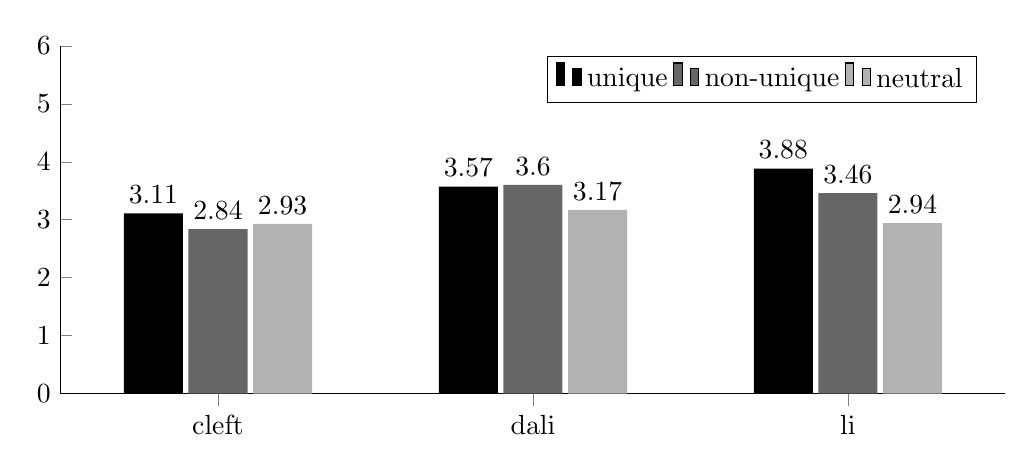
\begin{tikzpicture}
    \begin{axis}[
	axis lines*=left,
    width  = .6\textwidth,
	height = 6cm,
	nodes near coords,
    nodes near coords style={text=black},
	ymin=0,
	ymax=6,
	ytick distance=1,
	xtick=data,
	legend pos=north east,
	legend columns=-1,
    enlarge x limits=0.25,
	bar width=.75cm,
	x=4cm,
	x tick label style={align=center,text width=1cm},
	ybar,
	xticklabels={cleft,dali,li}
	]
  \addplot[fill=black,draw=none] coordinates {%feel free to also use other colors than black
    (1,3.11)    % cleft
    (2,3.57)    % dali
    (3,3.88)    % li
  };
    \addplot[fill=black!60,draw=none] coordinates {
    (1,2.84)    % cleft
    (2,3.6)     % dali
    (3,3.46)    % li
  };
    \addplot[fill=black!30,draw=none] coordinates {
    (1,2.93)    % cleft
    (2,3.17)    % dali
    (3,2.94)    % li
  };
  \legend{unique, non-unique, neutral}
    \end{axis}
  \end{tikzpicture}
    \caption{Overall ratings}
    \label{overall}
\end{figure}

The responses were analyzed with a mixed ANOVA, using the RStats package \citep{Rstats}. The factors were \textsc{question type} (3 levels: XP-LiQ, DaliQ, CleftQ) and  \textsc{context type} (3 levels: Unique\,+\,Surprise, Non-unique\,+\,Surprise and Neutral). The test revealed significant effects of \textsc{question type}, \textsc{context type}, and the combination of \textsc{question type} and \textsc{context type}. This lead us to follow up with pairwise comparisons (one-way ANOVA, again using RStats) between these factors, focussing on the drawn hypotheses. The comparison of \textit{li} and \textit{dali} in unique and non-unique contexts is plotted in \figref{dalipic}.

% Figure 2

\begin{figure}
  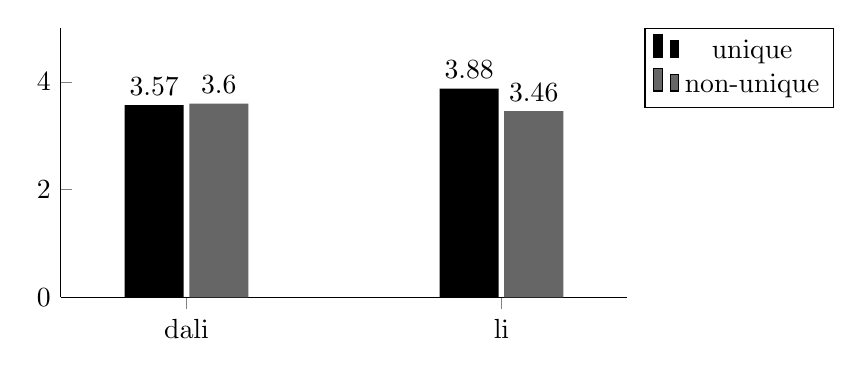
\begin{tikzpicture}
    \begin{axis}[
	axis lines*=left,
    width  = .6\textwidth,
	height = 5cm,
	nodes near coords,
    nodes near coords style={text=black},
	ymin=0,
	ymax=5,
	xtick=data,
	legend pos=outer north east,
	enlarge x limits=0.4,
	bar width=.75cm,
	x=4cm,
	x tick label style={align=center,text width=1cm},
	ybar,
	xticklabels={dali,li}
	]
  \addplot[fill=black,draw=none] coordinates {%feel free to also use other colors than black
    (1,3.57)     % dali unique
    (2,3.88)     % li unique
  };
    \addplot[fill=black!60,draw=none] coordinates {
    (1,3.6)     % dali non-unique
    (2,3.46)     % li non-unique
  };
  \legend{unique, non-unique}
    \end{axis}
  \end{tikzpicture}
    \caption{\textit{li} v. \textit{dali}}
    \label{dalipic}
\end{figure}


No significant differences between \textit{li} and \textit{dali} were found between unique or non-unique contexts. This suggests that uniqueness does not have an effect on the rating of the use of \textit{li} or \textit{dali} in a question.

In \figref{lipic} the results of the ratings of \textit{li} questions in Unique\,+\,Surprise, Non-unique\,+\,Surprise and Neutral contexts are plotted.

% Figure 3

\begin{figure}
  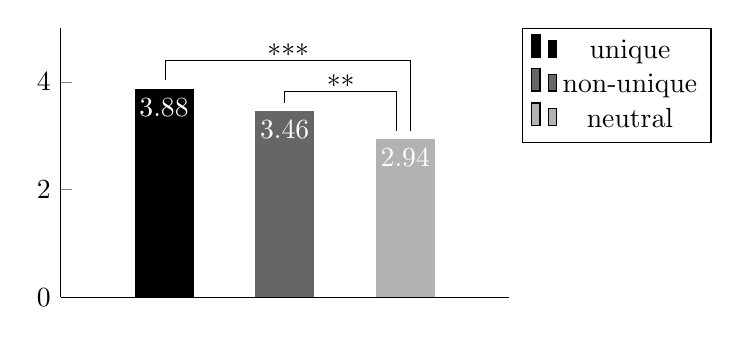
\begin{tikzpicture}
    \begin{axis}[
	axis lines*=left,
    width  = .6\textwidth,
	height = 5cm,
	nodes near coords,
    nodes near coords align={anchor=north, below},
    nodes near coords style = {color=white},
	ymin=0,
	ymax=5,
	xmajorticks = false,
	legend pos=outer north east,
    bar width=.75cm,
    enlarge x limits=1.5,
	x tick label style={align=center,text width=1cm},
	ybar,
	xticklabels={li}
	]
    \addplot[fill=black,draw=none]
    coordinates   {%feel free to also use other colors than black
     (0,3.88)   % li unique
  };
    \addplot[fill=black!60,draw=none] coordinates  {
    (1,3.46)     % li non-unique
  };
    \addplot[fill=black!30,draw=none] coordinates {
    (2,2.94)     % li neutral
  };
  \draw (axis cs:-1.125,4.03) |- ++(0,2.5mm) -| (axis cs:3.25,3.09) node [near start,above=-5pt] {***};
  \draw (axis cs:1,3.61) |- ++(0,1.5mm) -| (axis cs:3,3.09) node [near start,above=-5pt] {**};
  \legend{unique, non-unique, neutral}
    \end{axis}
  \end{tikzpicture}
    \caption{\textit{li} across contexts}
    \label{lipic}
\end{figure}

The results reveal that XP-LiQs get significantly higher ratings in surprise contexts. There is a significant difference between the ratings of XP-LiQs in Surprise\,+\,Unique contexts and Neutral contexts ($p<0.005$), as well as between the ratings in Surprise\,+\,Non-unique contexts and Neutral contexts ($p<0.05$). XP-LiQs get significantly higher ratings in surprise contexts across the board.

An anonymous reviewer pointed out to us that uniqueness seems to play a role in the licensing of \textit{li}, because the significance of the effect is higher for Unique\,+\,Surprise than for
Non-Unique\,+\,Surprise. As suggested by the same reviewer, we applied a two-factor ANOVA (using the RStats package) to the two relevant context types: Unique\,+\,Surprise and Non-Unique\,+\,Surprise. This test revealed no significant differences between the rankings of XP-LiQs and DaliQs in these contexts.

Finally, we did not find any significant differences between speakers of the different dialect groups. Because the sample size of this study was too small to draw conclusions from this result, we leave the issue of regional variation for future research.

%%%%%%%%%%%%%%%%%%%%%%%%%%%%%%%%%%%%%%%%%

\subsection{Discussion}\label{sec:discussion}
Let us turn to the implications of the data now and evaluate the results in the light of the drawn hypotheses.

First, consider hypothesis 1 in which we hypothesized that XP-LiQs signal that the property (or entity) that is denoted by the \textit{li}-marked constituent is unique. If this is the case, we expect XP-LiQs to get better ratings in unique contexts, compared to non-unique contexts. We found no significant differences between the ratings of XP-LiQs in unique and non-unique contexts ($p=0.10$). Furthermore, hypothesis 1 predicts that DaliQs are rated better in non-unique contexts than XP-LiQs, which is not the case, as illustrated in \figref{overall} ($p=0.50$). Finally, a two-factor ANOVA did not show an effect of uniqueness. We take this as evidence against hypothesis 1. We do, however, acknowledge that the significance of the effect is higher for Unique\,+\,Surprise than for Non-Unique\,+\,Surprise. One could speculate that there is an interaction between the factors. At this point, we leave this for further research.

Secondly, let us turn to hypothesis 2 claiming a correlation between XP-LiQs and the speaker being surprised about the property (or entity) that is denoted by the \textit{li}-marked constituent. This would predict better ratings for XP-LiQs in surprise contexts, both unique and non-unique, as compared to neutral contexts. This prediction is borne out: XP-LiQs got significantly better ratings in surprise than in neutral contexts. We take this to be a solid argument in favour of hypothesis 2.
%%%%%%%%%%%%%%%%%%%%%%%%%%%%%%%%%%%%%
%       Section 5
%%%%%%%%%%%%%%%%%%%%%%%%%%%%%%%%%%%%%
\section{General discussion}\label{sec:analysis}
We now turn to the general implications of the results in \sectref{sec:diss} and follow the discussion up with open issues in \sectref{sec:oi}. The nature of the discussion is exploratory, as it is beyond the aim of this paper to offer a full analysis of XP-LiQs. Specifically, we investigate the idea that the attested surprise effect is derived from general pragmatic principles as a result of focus marking, by the attachment of \textit{li} to a constituent.

\subsection{Discussion of hypothesis 2}\label{sec:diss}
At this point, a tempting route to explore the theoretical mechanism behind the `surprise' hypothesis would be to analyze \textit{li} as a mirative particle. It has long been known that there are languages, e.g. \ili{Japanese} and languages from the Amazonia and Himalayas, that mark a surprised feeling using particles \citep{sudo2013,DeLancey2012}. These particles are referred to as mirative particles. There are various definitions of mirativity available in the literature and it is beyond the scope of this paper to contribute to this debate. Having said that, there is consensus about the idea that mirative marking indicates that the expressed proposition is not part of the propositional content that the speaker has at her disposal, based on background knowledge or previous establishments of the truth of the proposition \citep{DeLancey2012,Donabedian2001}. We found that XP-LiQs are more felicitous in contexts where the speaker is surprised, suggesting it could be analyzed as a mirative particle.

\begin{sloppypar}
We have two main arguments against analyzing \textit{li} as a marker of mirativity. %First of all, it is known that mirative particles are very rare in indo-european languages.
First of all, the particle \textit{li} occurs in many \ili{Slavic} languages and it has been ana\-lyzed as associating with focus in the languages in which it occurs \citep{schwabe2004}. While the usage of \textit{li} is subject to variation -- for example \ili{Bulgarian} can have sentence-final \textit{li} questions which are interpreted as neutral \citep{dukova2010}, while \textit{li} in \ili{Czech} is only found in conditionals \citep{schwabe2004} -- it would be remarkable if \textit{li} were a plain surprise particle in one \ili{Slavic} language and something else in a different one.
\end{sloppypar}

Secondly, if \textit{li} were a mirativity marker, we would predict it to mark surprise across the board, including, for example, conditionals like \REF{nosurprise}.

% Example 12

\ea \gll Mine li, gori zemja-ta. \\
pass.by.\textsc{prs.3sg} \textsc{li} burn.\textsc{prs.3sg} earth-\textsc{def.sg.f} \\ \hfill habitual conditional
\glt `Whenever/if (s)he walks by, the earth burns.'\hfill \citep[539]{koneski1987}\label{nosurprise}
\z

\noindent
This prediction is not borne out, i.e., in \REF{nosurprise}, there is no surprise effect. As suggested by an anonymous reviewer, \textit{li} being a focus marker, however, is compatible with \REF{nosurprise},
%\Last,
as the focus can generate the alternatives `(S)he passes' and `(S)he doesn't pass', one of which is then picked as the condition for the apodosis.

Therefore, we explore an alternative explanation of our finding that surprise increases the felicity of XP-LiQs. Namely, that this is a result of a more general pragmatic principle.

As we pointed out in \sectref{sec:back}, traditionally, \textit{li} has been analyzed as a focus particle in questions. Based on \citet{Meertens.Egger.Romero2018}, who propose an analysis for the \ili{Turkish} question particle \textit{mI}, we take two ingredients from the literature, namely (i) the hierarchical organization of discourse in QUDs  \citep{Roberts2012,Buering2003} and (ii) focus (F-)marking \citep{rooth1992}. \citet{Roberts2012} proposes that the shape of the QUD is determined by the placement of F-marking. Along the lines of \citet{Meertens.Egger.Romero2018}, we propose that the placement of \textit{li} determines the shape of the QUD. Let us first illustrate how such an analysis works and then turn to the surprise effect.

First, let us take discourse structure to consist of QUDs, which produces a set of hierarchically ordered questions, as in \figref{roberts8}.\largerpage

% Example 13

%\ea \label{roberts8}
%\hbox{\scriptsize{
%\Tree [.{Who ate what?} [{Did Amy eat tofu?} {Did Amy eat natto?} ... ].{What did Amy eat?} [ {Did Bob eat tofu?} {Did Bob eat natto?} ... ].{What did Bob eat?} ]}}
%\z

\begin{figure}
    \small
    \begin{forest}for tree={l=1.5cm}
[{Who ate what?}, s sep=1cm
    [{What did Amy eat?}
    [{Did Amy\\eat tofu?}]
    [{Did Amy\\eat natto?}, before computing xy={s/.average={s}{siblings}}]
    [{\dots} ] ]
        [{What did Bob eat?}
        [{Did Bob\\eat tofu?}]
        [{Did Bob\\eat natto?}, before computing xy={s/.average={s}{siblings}}]
        [{\dots} ] ]
]
\end{forest}
    \caption{QUD-tree\label{roberts8}}
\end{figure}

Secondly, we take \citeposst{rooth1992} analysis of focus. An utterance has an ordinary semantic value and a focus semantic value \sib{$\phi$}$^f$, consisting of a set of alternatives of the focus-marked element. An example is given in \REF{focus value}. The notation \sib{$\phi$}$^f$ stands for the focus alternatives of $\phi$ and $C$ stands for the semantically closest alternative. The felicity condition of the squiggle operator $\sim$ is defined in \REF{focus felicity}.



% Example 14

\begin{exe}
\ex \begin{xlist}
\ex\label{focus value} \sib{Ali\textsubscript{F} played cards}$^{f} =$\\ \{a played cards, b played cards, c played cards, {\dots}\}
\ex\label{focus felicity} \sib{$\phi \sim C$} is felicitous only if \sib{$C$} $\subseteq$ \sib{$\phi$}$^f$
\end{xlist}
\end{exe}

\noindent We follow \citet{Roberts2012} and \citet{biezma2009} and take the location of focus marking to constrain the shape of the immediate QUD. For the sentence \textit{Did Amy eat tofu?}, for example, the placement of focus determines whether the immediate QUD is questioning the subject or the object of the utterance. Focus on the subject signals that the immediate QUD questions the subject, whereas focus on the object signals that the immediate QUD questions the object, as illustrated in Figures~\ref{ex:biezma1} and \ref{ex:biezma2}.

% Example 15

%\begin{exe}
%\ex \label{ex:biezma1}{\footnotesize
%\Tree [.{QUD: Who ate tofu?} {Did AMY$_F$ eat tofu?} {Did BOB$_F$ eat tofu?} {...} ]}

\begin{figure}\small
\begin{forest}
for tree={s sep=1.6cm, inner sep=0.1cm, l=2cm}
[QUD: Who ate tofu?
    [Did \emph{Amy}\textsubscript{F} eat tofu?]
    [Did \emph{Bob}\textsubscript{F} eat tofu?, before computing xy={s/.average={s}{siblings}}]
    [{\dots}]
]
\end{forest}
\caption{Subject focus QUD-tree\label{ex:biezma1}}
\end{figure}

% Example 16

%\ex \label{ex:biezma2}{\footnotesize
%\Tree [.{QUD: What did Amy eat?} {Did Amy eat TOFU$_F$?} {Did Amy eat NATTO$_F$?} {...} ]}
%\end{exe}

\begin{figure}\small
\begin{forest}
for tree={s sep=1cm, inner sep=0.1cm, l=2cm}
[QUD: What did Amy eat?
    [Did Amy eat \emph{tofu}\textsubscript{F}?]
    [Did Amy eat \emph{natto}\textsubscript{F}?, before computing xy={s/.average={s}{siblings}}]
    [{\dots}]
]
\end{forest}
\caption{Object focus QUD-tree\label{ex:biezma2}}
\end{figure}

Now, if we take \textit{li} to focus-mark the constituent it is adjacent to and thus to shape the QUD, certain predictions about the usage of focus in questions arise. It is expected that, for example, focus-marking the object (and thus indicating that the immediate QUD is questioning it) gives a special status to that object, as compared to other constituents in the sentence. In other words, narrow focus in a question is particularly compatible with certain contexts, among which surprise, as  \citet{bianchi.cruschina2016} found for \ili{Italian} and \ili{Italian} dialects. %that in \ili{Italian}, narrow focus, by means of focus fronting, in polar questions is indeed especially compatible with contexts in which the focused constituent has a special status, including contexts in which the speaker is surprised about the constituent.

It should be noted that a QUD analysis predicts, in principle, that XP-LiQs are felicitous in any context in which the speaker has a reason to shape the QUD in a particular way.
%is particularly interested in a specific consituent.
Let us briefly return to the results of our study. We listed the items that conveyed a feeling of \textsc{interest} in a specific constituent, as in, for example, \REF{interest}.

% Example 17

\eanoraggedright \label{interest}
\eanoraggedright \textit{Scenario}: Your sister has been watching the champions league final. It was Chelsea against Bayern München. You thought Bayern München would win, because they are a better team, but when you walk in the living room, your sister, wearing a Chelsea shirt, jumps up to hug you. You ask her:
\ex Chelsea-\textsc{li} won the Champions League? \hfill XP-LiQ
\ex Did Chelsea win the Champions League? \hfill DaliQ
\ex Is Chelsea the team that won the Champions League? \hfill CleftQ
\z\z

\noindent
In \REF{interest}, one can imagine that on top of the discrepancy between epistemic and evidential bias, the speaker also has a great interest in the outcome of the game. A post-hoc analysis of those examples did not show a trend or significant effect of interest on the rankings of \textit{li}. We leave this for further research.

Concluding this section, our finding is that the higher rating of XP-LiQs in surprise contexts as opposed to neutral ones is straightforwardly analyzed as the result of \textit{li}'s function as a focus marker, its effect being the shaping of the QUD.

\subsection{Open issues}\label{sec:oi}
In the remainder of our paper, we will discuss a number of open issues. The first issue is concerned with the various strategies of focus marking that \ili{Macedonian} has access to. In this paper, we concentrated on focus marking by the placement of \textit{li}. However, focus can also be marked by placing a focal accent on a constituent and by word order. It is far from clear what the interplay is between these strategies and a complete analysis of focus marking of \ili{Macedonian} needs to take all three into account.

%  \subsubsection{Differences between Macedonian and Bulgarian}
%  With varying degree of productivity, this particle can be found in questions and/or conditionals in most \ili{Slavic} languages \citet{schwabe2004particle}. While more work has been done on \textit{li} in \ili{Bulgarian} than on \ili{Macedonian}, note that there are some striking differences between the use of \textit{li} in \ili{Macedonian} and \ili{Bulgarian}.

%  First of all, \citet{dukova2010questions} states that for \ili{Bulgarian} \textit{li} is also felicitous in sentence final position, where it has a neutral polar question interpretation, see \REF{}. This is position is not available for \textit{li} in \ili{Macedonian} (\citep[55]{friedman2002macedonian}).

% Furthermore, \textit{li} in \ili{Bulgarian} can appear in embedded questions, while in \ili{Macedonian} this is marginal \citet{Rudin.Kramer.Billings.Baerman1999}, \citet{dukova2010questions}.

% Thirdly, V-\textit{li} questions in \ili{Bulgarian} can have a neutral reading \citep[179]{dukova2010questions}, whereas in \ili{Macedonian} they have a narrow focus  \citet{Rudin.Kramer.Billings.Baerman1999}.

% Fourthly, in her corpus study of \ili{Bulgarian} and \ili{Macedonian} literature \citet{englund1977yes} found that \ili{Macedonian} polar questions are formed with li in 30\% of the cases, whereas in \ili{Bulgarian} this was 60\%. Nikov (as cited in \citep[577]{Rudin.Kramer.Billings.Baerman1999}found in a corpus study that li is used in \ili{Bulgarian} in 92,2\% of the cases. On the other hand, IntQs are marginal in \ili{Bulgarian} \citet{Rudin.Kramer.Billings.Baerman1999} (though \citet{dukova2010questions} has shown that they are nonetheless felicitous).

An additional open issue is the fact that in the experiment, we only tested contexts in which there is a bias conflict. Such contexts are very compatible with a QUD that is shaped by narrow-focus marking. Recall that we interpreted these results as evidence for a focus account. Such an account also predicts licensing of \textit{li} in contexts that are compatible with focus marking for other reasons, such as in \REF{doubleask} from \citet{bianchi.bocci.cruschina2016}, in which the speaker is double checking the constituent she is focus-marking.

% Example 18

\eanoraggedright
\textit{Scenario}: Peppe is an architect. Whenever he works in his office he comes home at 6pm; whenever he has to go to the land registry office or the town hall instead, he comes home late.
\begin{xlist}
\exi{A:}{Peppe came home late today.}
\exi{B:}{Did he have to go to the \emph{townhall}?\hfill \citep{bianchi.bocci.cruschina2016}}
\end{xlist}\label{doubleask}
\z

\noindent
At this point, intuitions about examples like \REF{doubleask} in \ili{Macedonian} are unclear and the felicity of XP-LiQs in such a context needs to be tested empirically. We leave this issue for further research.

A final open issue is how polar questions with \textit{li} attached to the verb, such as \REF{topli} and \REF{vli}, rather than to an XP, are interpreted. While in \ili{Bulgarian}, these can be interpreted as neutral questions \citep{Rudin.Kramer.Billings.Baerman1999, dukova2010}, in \ili{Macedonian} the neutral way of forming questions is with \textit{dali}, \REF{dali}, and the verb in V-LiQs is focused. DaliQs in \ili{Bulgarian}, on the other hand, are not neutral. As mentioned in \sectref{sec:back}, it has been reported that V-LiQs also seem to convey a feeling of surprise. Whether this focus produces the same type of bias as what we have shown here for XP-LiQs remains for further research.

% \subsubsection{Excursus: what about the cleft questions? }
% While they were meant to match the unique context and be bad in the neutral and non-unique context, the cleft questions got the same rating across the board. Participants rated cleft questions around 3; the difference between contexts is not significant, as shown in Figure bla. We expected clefts to be significantly better in unique contexts. This result is unexpected, but not unprecedented. \citet{de2018s} found that certain participants consistently treated clefts as exhaustive (patterning with \textit{only}), whereas others treated them as non-exhaustive, as plain focus. Thus, clefts are not necessarily always interpreted as exhaustive or unique.

% Another possible explanation for the ratings of the cleft questions, is that these constructions are not frequently used in \ili{Macedonian}, this might have made some speakers unsure of their meaning. (why?)

% Lastly, cleft questions also have a version with \textit{li} and without \textit{li}, see \REF{cleftli}, further complicating things. (how?)

% \begin{exe} \ex
% \begin{xlist}
% \ex \gll Ti si taa na koj-a što i padna parička-ta? \\
% \textsc{2sg} be.\textsc{2sg.prs.nom} \textsc{3sg.f} on who-\textsc{f} what \textsc{3sg.f.dat} fall.\textsc{3sg.prs} coin.\textsc{dim-def.f} \\ \trans
% `Are you the one who got the coin?'
% \ex \gll Ti li si taa na koj-a što i padna parička-ta? \\
% \textsc{2sg} \textsc{li} be.\textsc{2sg.prs.nom} \textsc{3sg.f} on who-\textsc{f} what \textsc{3sg.f.dat} fall.\textsc{3sg.prs} coin.\textsc{dim-def.f} \\ \trans `Are YOU the one who got the coin?'
% \end{xlist}
% \end{exe} \label{cleftli}

% We leave this open for now, as the interpretation of \textit{li} across contexts does not hinge on this.

\section{Conclusion}\label{j:sec:conclusion}

We presented an empirical study the results of which show that XP-LiQs are felicitous in contexts where there is surprise of the speaker about the property or entity that is denoted by the constituent that \textit{li} is attached to. The surprise was expressed in the contexts as a contrast between a negative epistemic and a positive evidential bias. We interpreted this result by proposing that this is a pragmatic effect of the focus marking done by \textit{li}: it focuses that constituent and in that way shapes the QUD.

\section*{Abbreviations}

\begin{tabularx}{.5\textwidth}{@{}lX}
\textsc{1, 2, 3}&first, second, third person\\
\textsc{cop}&{copula}\\
\textsc{def}&{definite}\\
\textsc{f}&{feminine}\\
\textsc{F}&{focus}\\
\end{tabularx}%
\begin{tabularx}{.5\textwidth}{lX@{}}
\textsc{m}&{masculine}\\
\textsc{pl}&{plural}\\
\textsc{prs}&{present tense}\\
\textsc{q}&{question particle}\\
\textsc{sg}&singular\\
\end{tabularx}

\section*{Acknowledgements}

We thank Magdalena Čačorovska, Marija Kocevska, Marjana Vaneva and especially Vasilija Šarac for their help with the \ili{Macedonian} judgments and with testing and distributing the survey. We also thank Muriel Assmann, Andrea Beltrama, Daniel Büring, Max Prüller, Maribel Romero, Catherine Rudin, the audience at FDSL\,13 and two anonymous reviewers for valuable comments and feedback. This work was supported by the Deutsche Forschungsgemeinschaft (\ili{German} Research Foundation) within project RO 4247/4-2 ``Alternativfragen'' of the FOR2111 ``Questions at the Interfaces'' and by the Austrian Science Fund (FWF), project grant P29180-G23, ``Unalternative Constraints Crosslinguistically''.

{\sloppy\printbibliography[heading=subbibliography,notkeyword=this]}

\end{document}
